\subsection{乱数生成の結果}

\subsubsection{一様乱数の生成結果}
一様乱数の結果を図\ref{fig:uniform-random}に示す。
$N$は生成した乱数の数であり、横軸が生成された乱数の値、縦軸がその頻度を示している。
$N$が最も小さいときは、頻度が一様とはいえないが、
$N$が大きくなるにつれ頻度が一様に近づいていることがわかる。
図\ref{fig:uniform-1Dpl}は横軸が生成回、縦軸が生成された乱数の値を示している。
一様乱数であるから特に規則性は見られず、0から1の間でランダムに値が生成され振動している様子がわかる。
図\ref{fig:uniform-2Dpl}は横軸が奇数回に生成された乱数、縦軸が偶数回に生成された乱数を示している。
図\ref{fig:uniform-1Dpl}と同様に規則性は見られず一様に分布している様子がわかる。
\begin{figure}
	\centering
	\begin{subfigure}{0.48\linewidth}
		\centering
		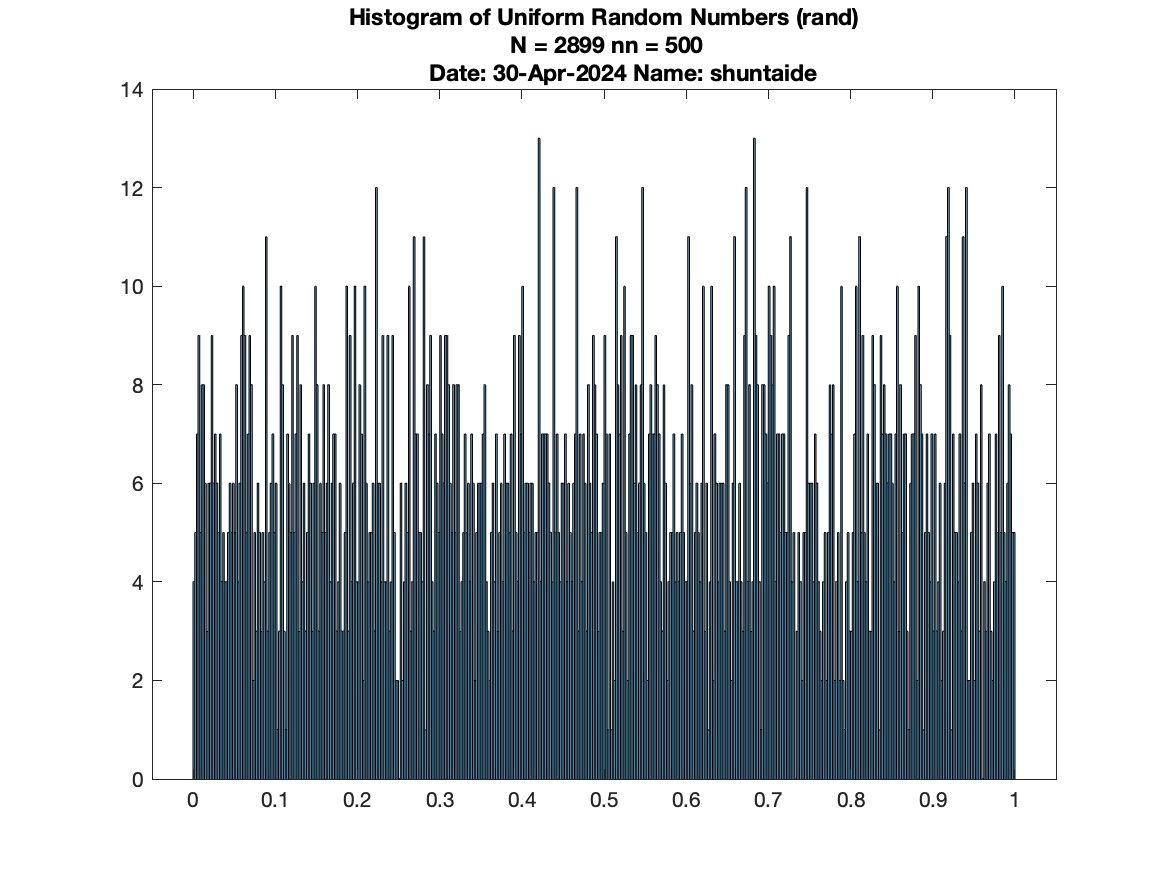
\includegraphics[width=0.8\textwidth]{src/figures/uniform/rand_hist_N=2899_nn=500.jpg}
		\subcaption{$N=2899$, $nn=500$}
	\end{subfigure}
	\begin{subfigure}{0.48\linewidth}
		\centering
		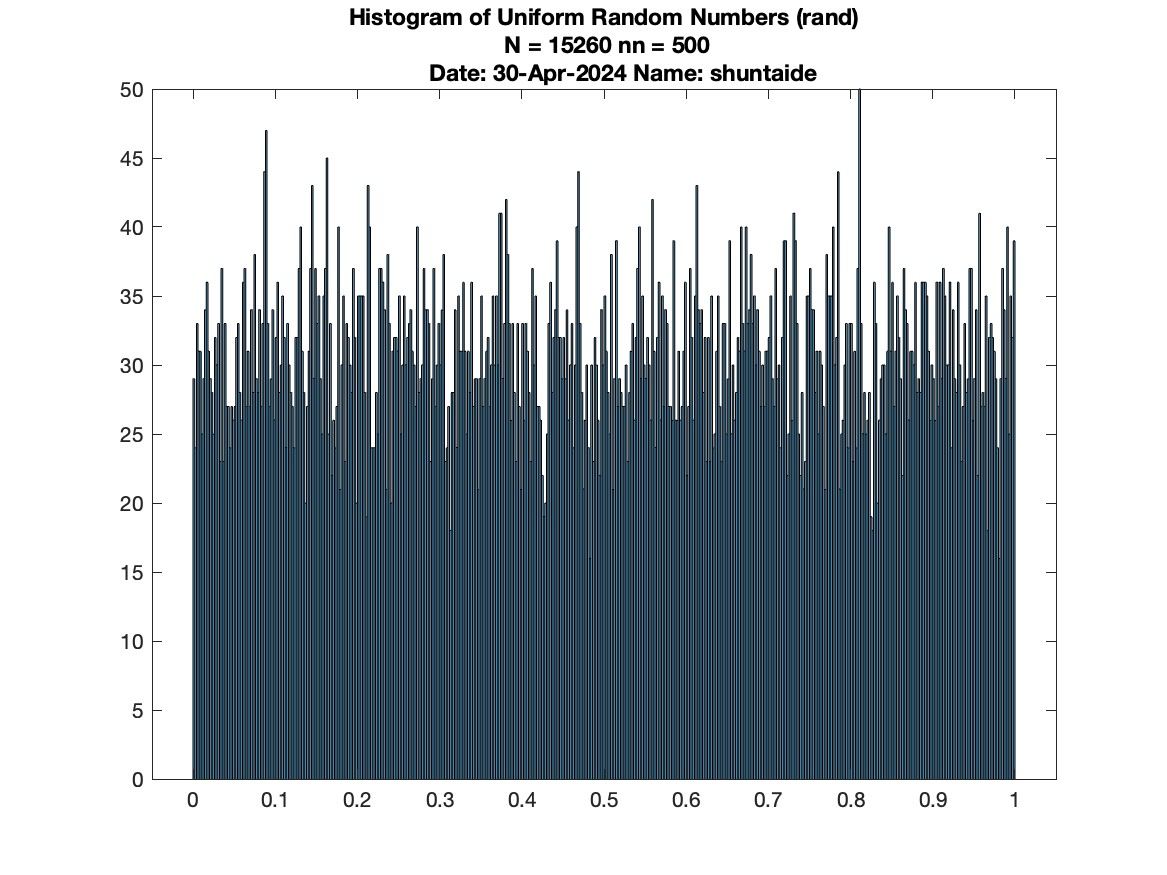
\includegraphics[width=0.8\textwidth]{src/figures/uniform/rand_hist_N=15260_nn=500.jpg}
		\subcaption{$N=15260$, $nn=500$}
	\end{subfigure}
	\begin{subfigure}{0.48\linewidth}
		\centering
		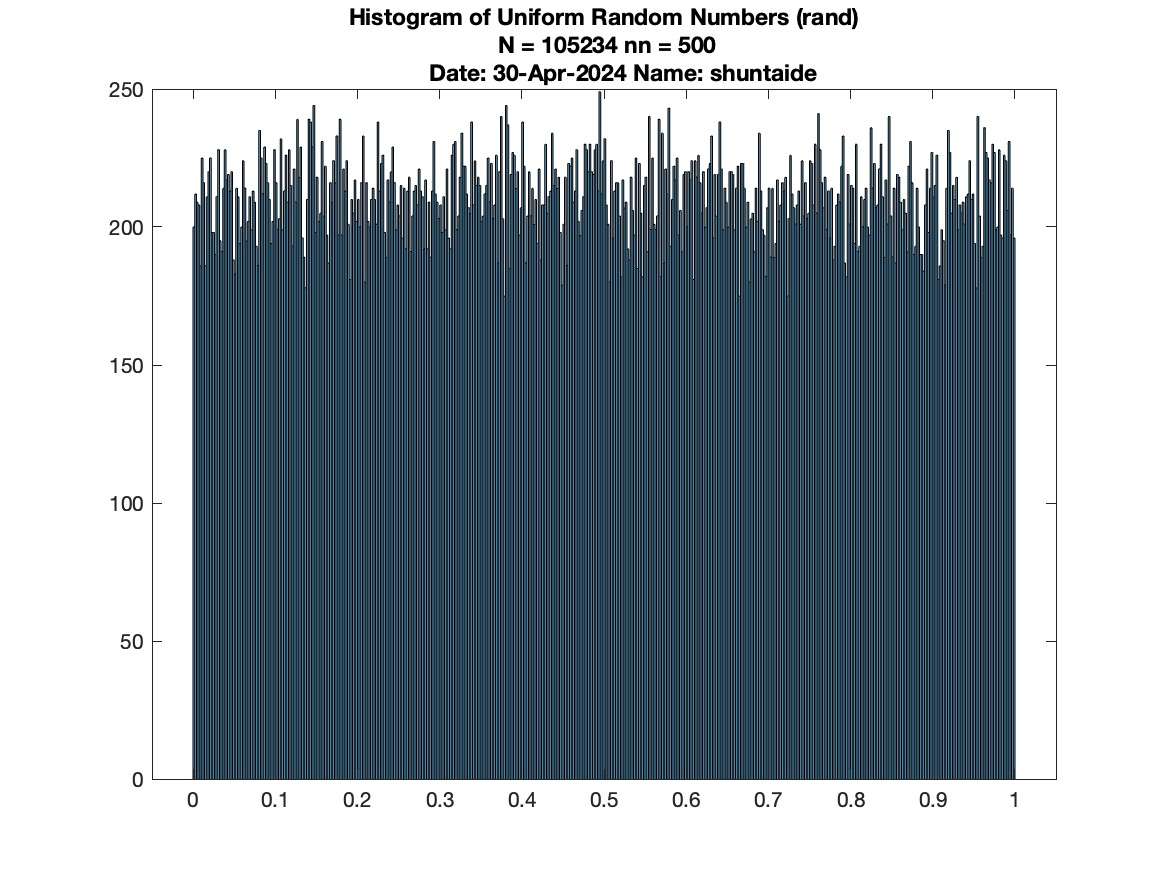
\includegraphics[width=0.8\textwidth]{src/figures/uniform/rand_hist_N=105234_nn=500.jpg}
		\subcaption{$N=105234$, $nn=500$}
	\end{subfigure}
	\begin{subfigure}{0.48\linewidth}
		\centering
		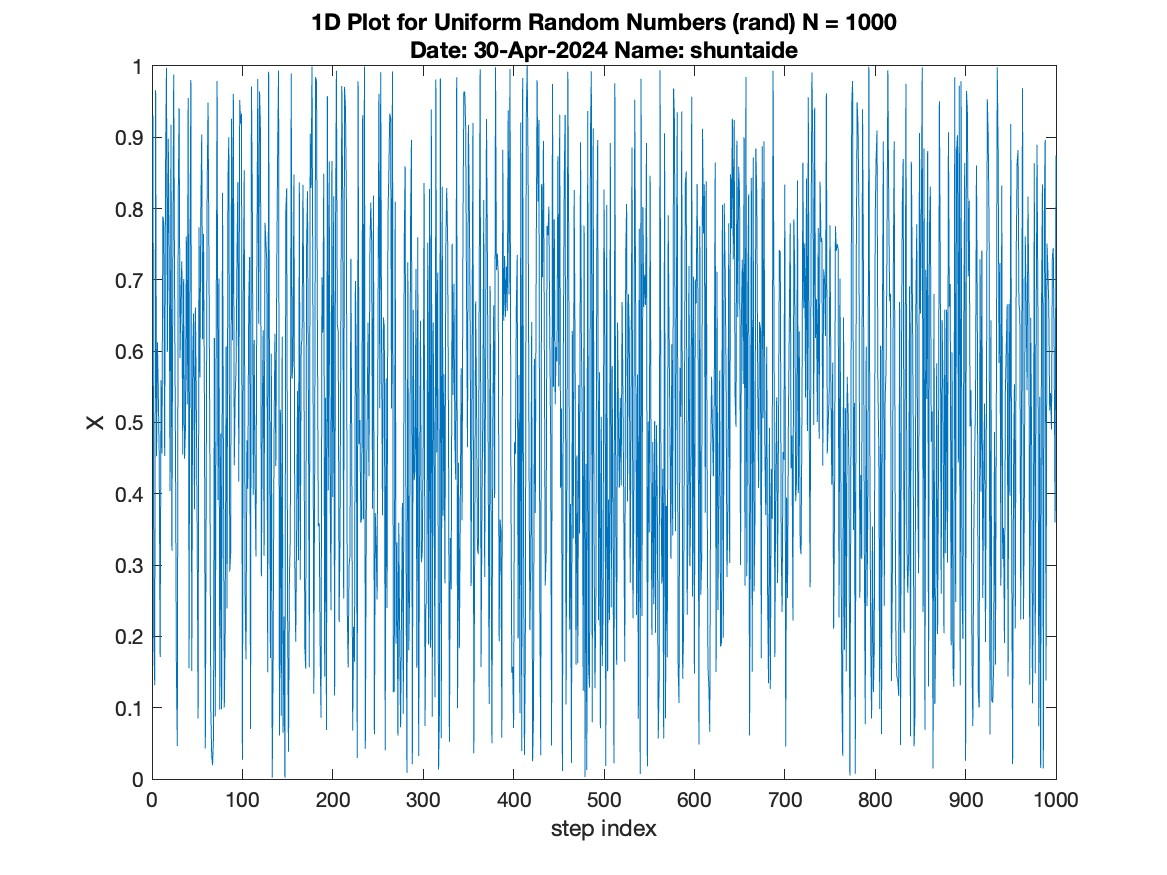
\includegraphics[width=0.8\textwidth]{src/figures/uniform/rand_1Dpl_N=1000.jpg}
		\subcaption{生成回と値の関係}\label{fig:uniform-1Dpl}
	\end{subfigure}
	\begin{subfigure}{0.48\linewidth}
		\centering
		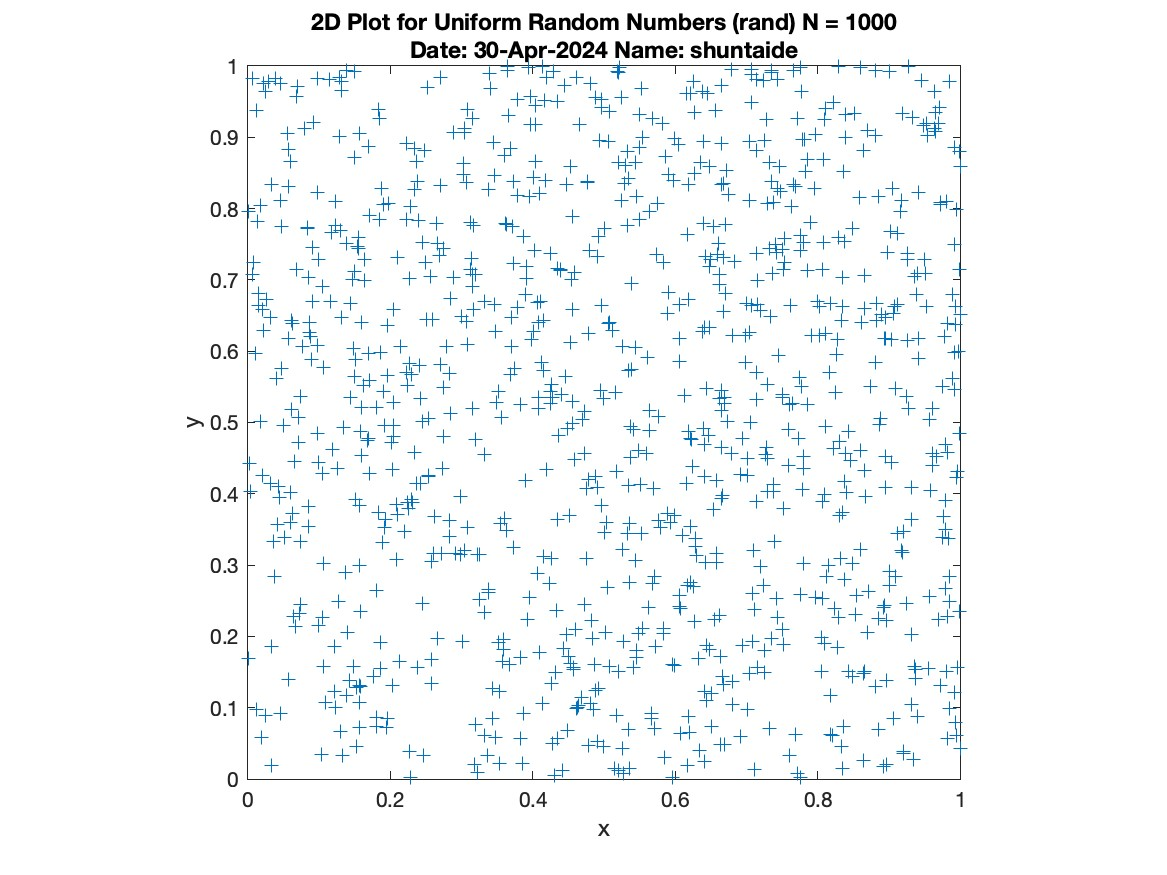
\includegraphics[width=0.8\textwidth]{src/figures/uniform/rand_2Dpl_N=1000.jpg}
		\subcaption{横軸が奇数回に生成された値、縦軸が偶数回に生成された値}\label{fig:uniform-2Dpl}
	\end{subfigure}
	\caption{一様乱数の生成結果}\label{fig:uniform-random}
\end{figure}


\subsubsection{標準正規乱数の生成結果}\label{subsubsec:standard-normal-random}
標準正規乱数の生成結果を図\ref{fig:standard-normal-random}に示す。
$N$は生成した乱数の数であり、横軸が生成された乱数の値、縦軸がその頻度を示している。
$N$が最も小さいときは、頻度が$0.5$付近が大きくそれから離れるにつれ小さくなっている様子がわかるが、
標準正規分布とは言いづらい。
$N$が大きくなるにつれ、形が標準正規分布に近づいていることがわかる。
図\ref{fig:standard-normal-1Dpl}は、横軸が生成回、縦軸が生成された乱数の値を示している。
一様乱数の図\ref{fig:uniform-1Dpl}と比べると、標準正規乱数は0付近に集中していることがわかる。
図\ref{fig:standard-normal-2Dpl}は、横軸が奇数回に生成された乱数、縦軸が偶数回に生成された乱数を示している。
図\ref{fig:standard-normal-1Dpl}と同様に0付近に集中していることがわかる。
図\ref{fig:uniform-2Dpl}と比べて中心に集中していることがわかる。
\begin{figure}
    \centering
    \begin{subfigure}{0.48\linewidth}
        \centering
        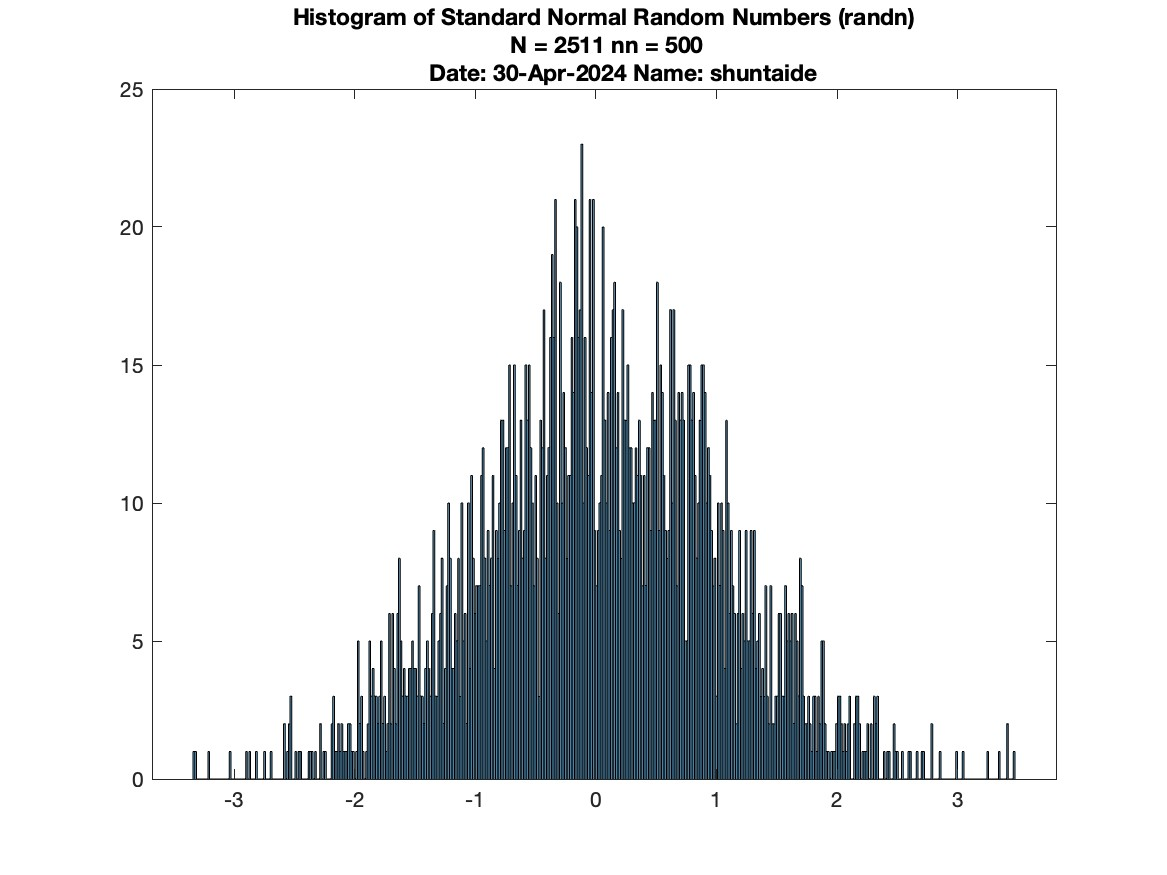
\includegraphics[width=0.8\textwidth]{src/figures/standard-normal/randn_hist_N=2511_nn=500.jpg}
        \subcaption{$N=2511$, $nn=500$}
    \end{subfigure}
    \begin{subfigure}{0.48\linewidth}
        \centering
        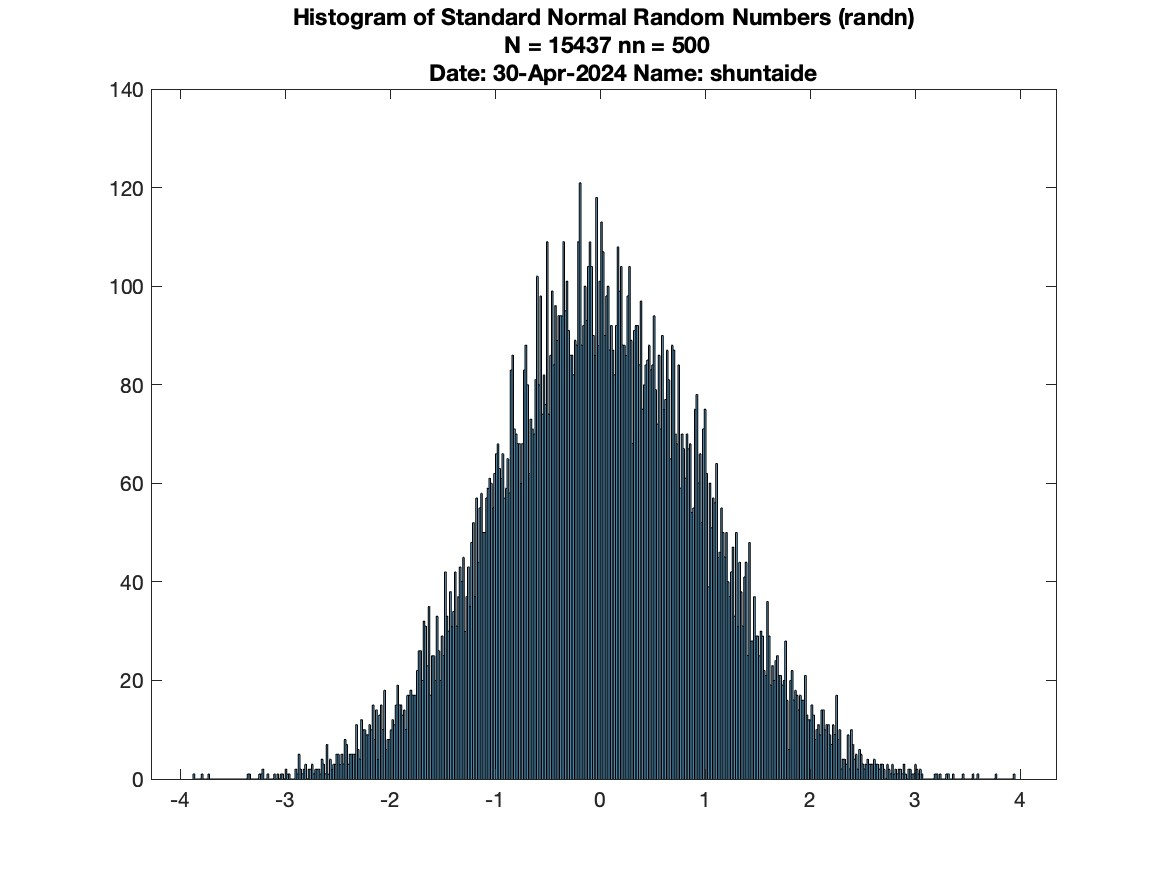
\includegraphics[width=0.8\textwidth]{src/figures/standard-normal/randn_hist_N=15437_nn=500.jpg}
        \subcaption{$N=15437$, $nn=500$}
    \end{subfigure}
    \begin{subfigure}{0.48\linewidth}
        \centering
        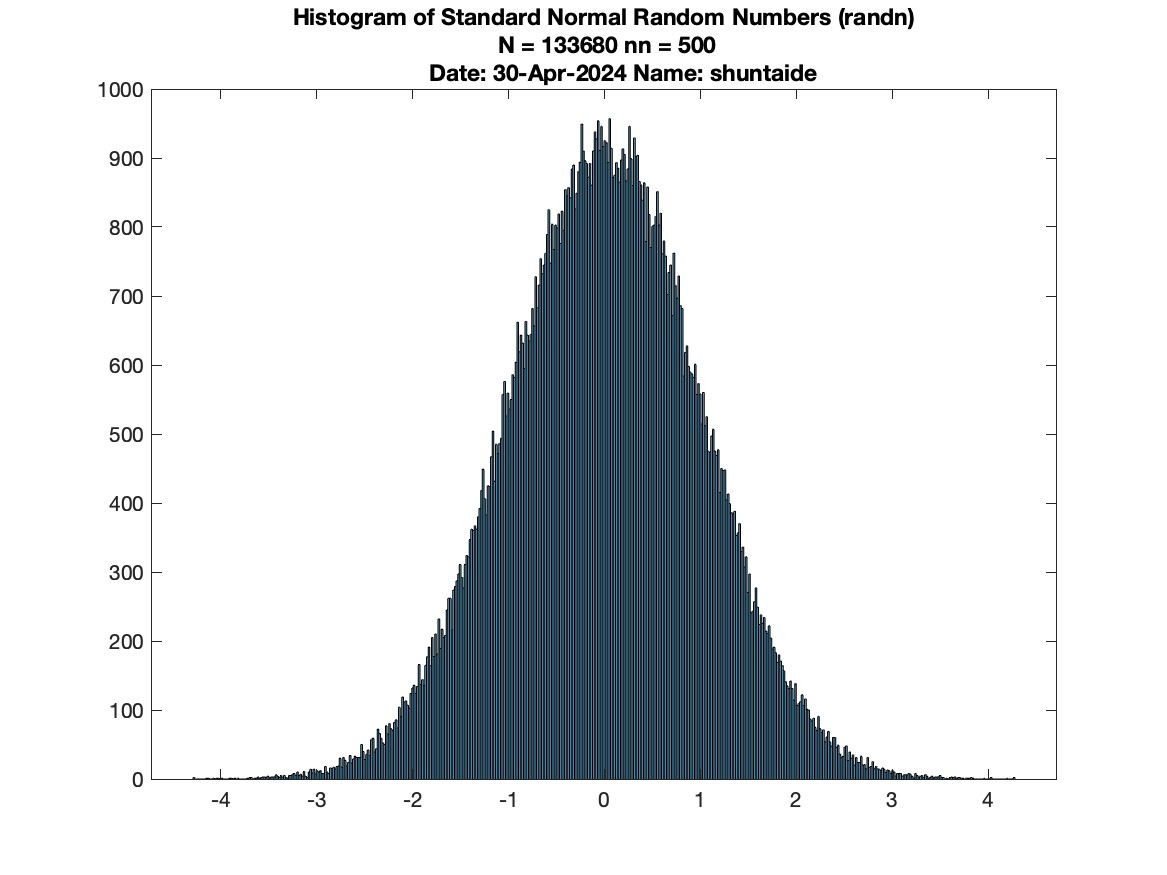
\includegraphics[width=0.8\textwidth]{src/figures/standard-normal/randn_hist_N=133680_nn=500.jpg}
        \subcaption{$N=133680$, $nn=500$}
    \end{subfigure}
    \begin{subfigure}{0.48\linewidth}
        \centering
        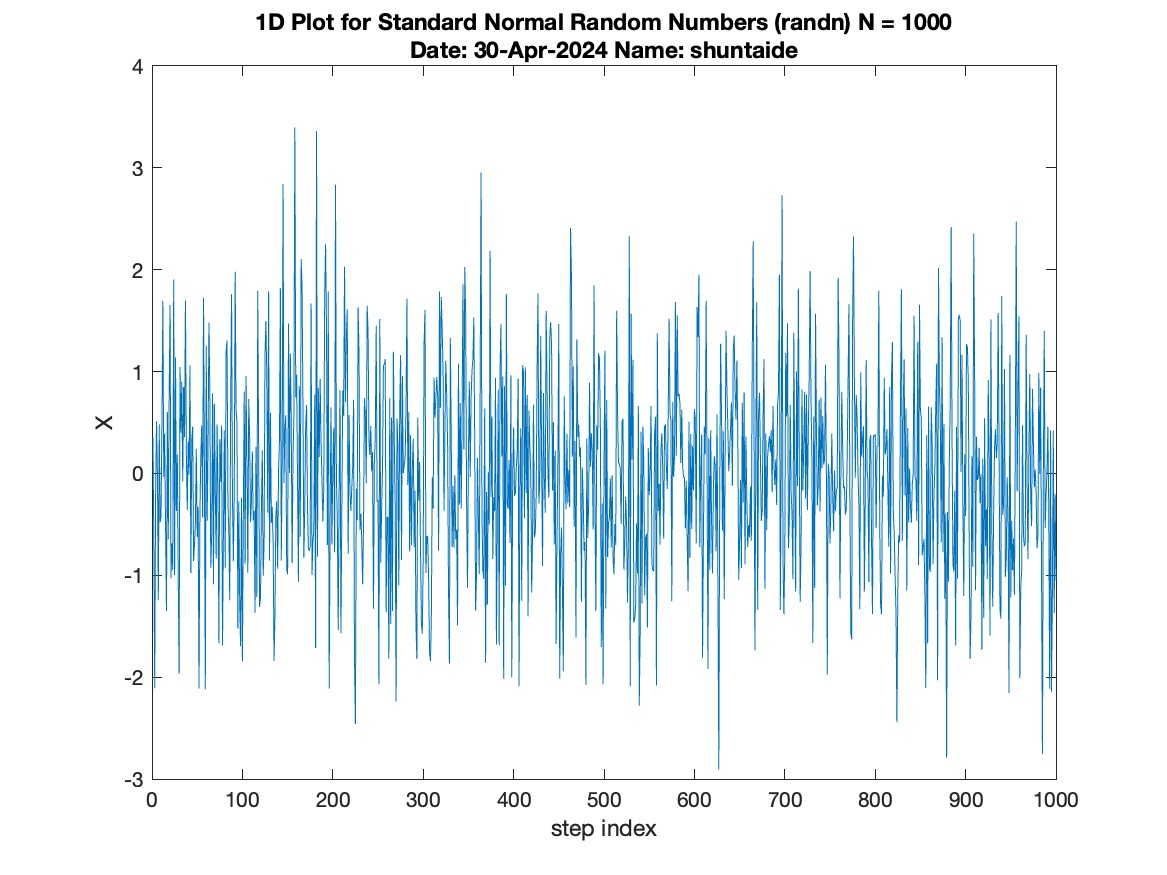
\includegraphics[width=0.8\textwidth]{src/figures/standard-normal/randn_1Dpl_N=1000.jpg}
        \subcaption{生成回と値の関係}\label{fig:standard-normal-1Dpl}
    \end{subfigure}
    \begin{subfigure}{0.48\linewidth}
        \centering
        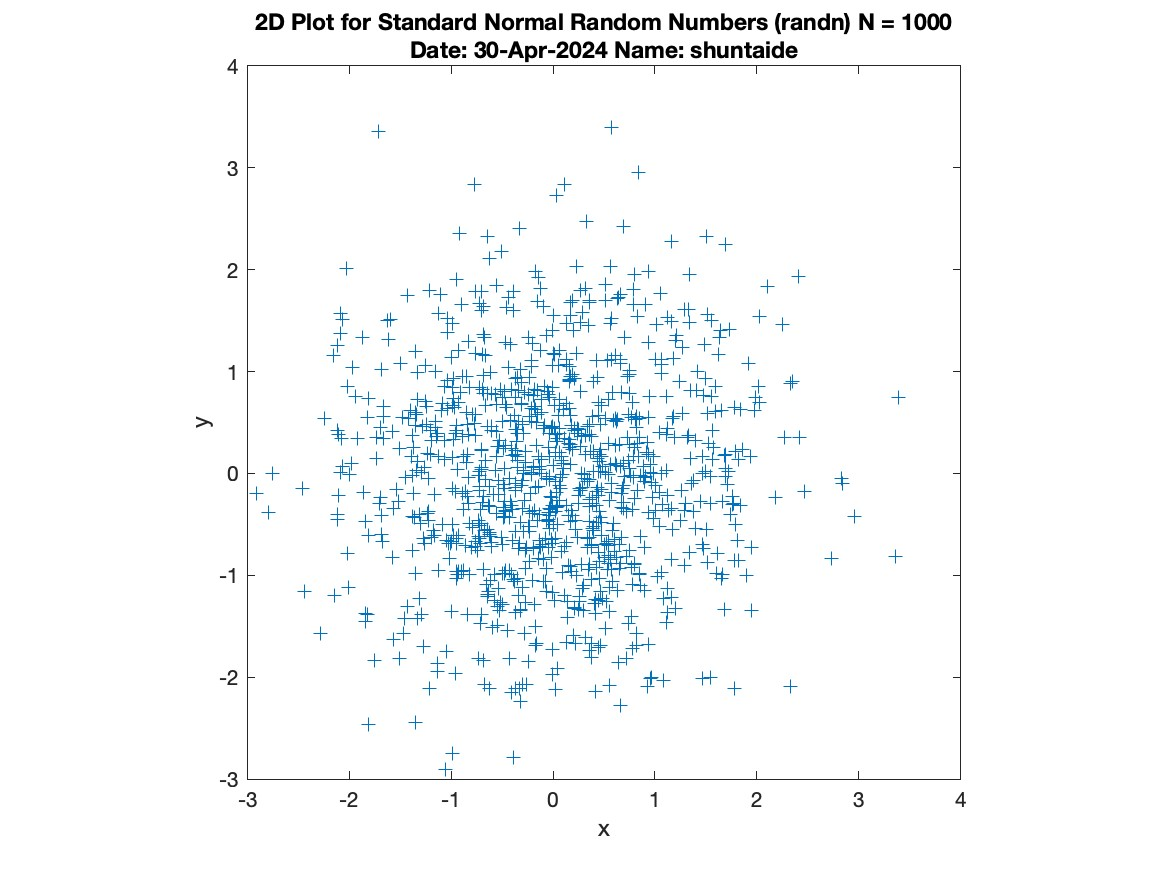
\includegraphics[width=0.8\textwidth]{src/figures/standard-normal/randn_2Dpl_N=1000.jpg}
        \subcaption{横軸が奇数回に生成された値、縦軸が偶数回に生成された値}\label{fig:standard-normal-2Dpl}
    \end{subfigure}
    \begin{subfigure}{0.48\linewidth}
        \centering
        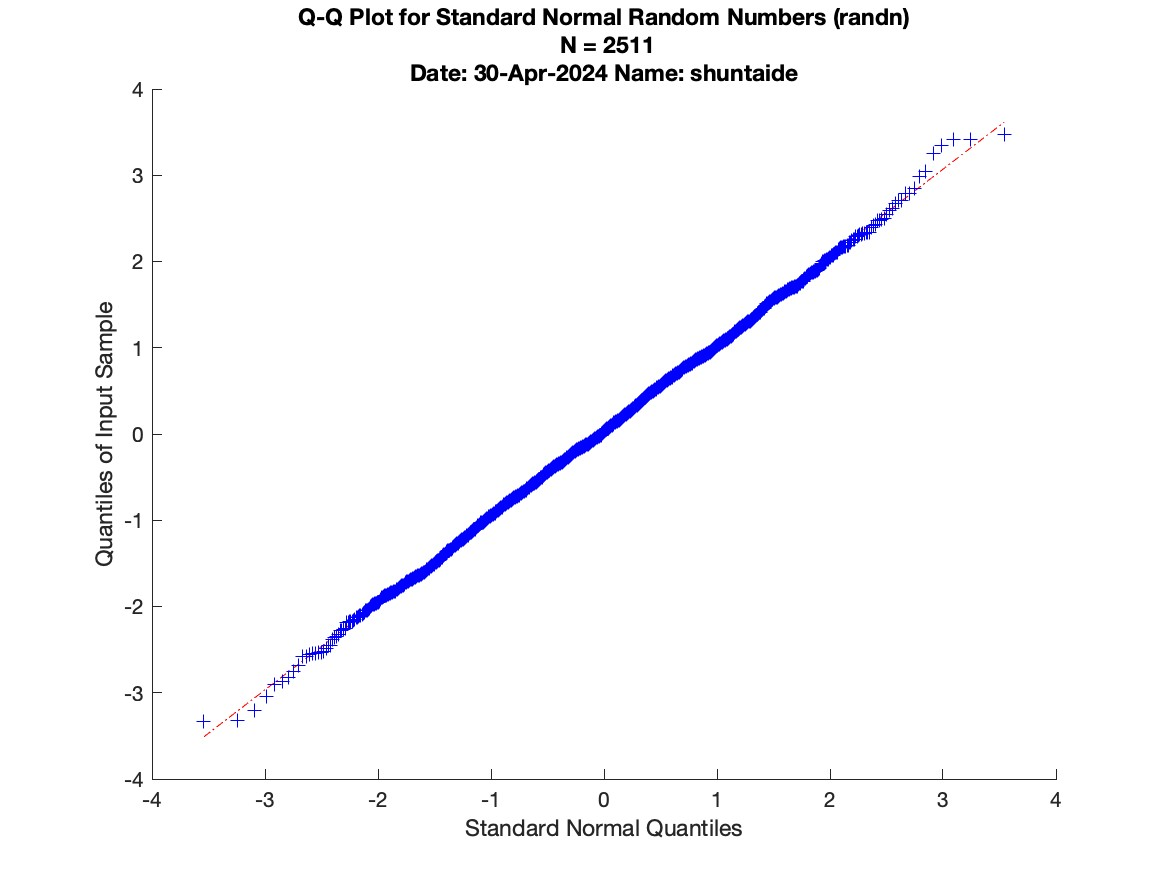
\includegraphics[width=0.8\linewidth]{src/figures/standard-normal/randn_qqpl_N=2511.jpg}
        \subcaption{QQプロット($N=2511$)}\label{fig:standard-normal-qqpl-2511}
    \end{subfigure}
    \begin{subfigure}{0.48\linewidth}
        \centering
        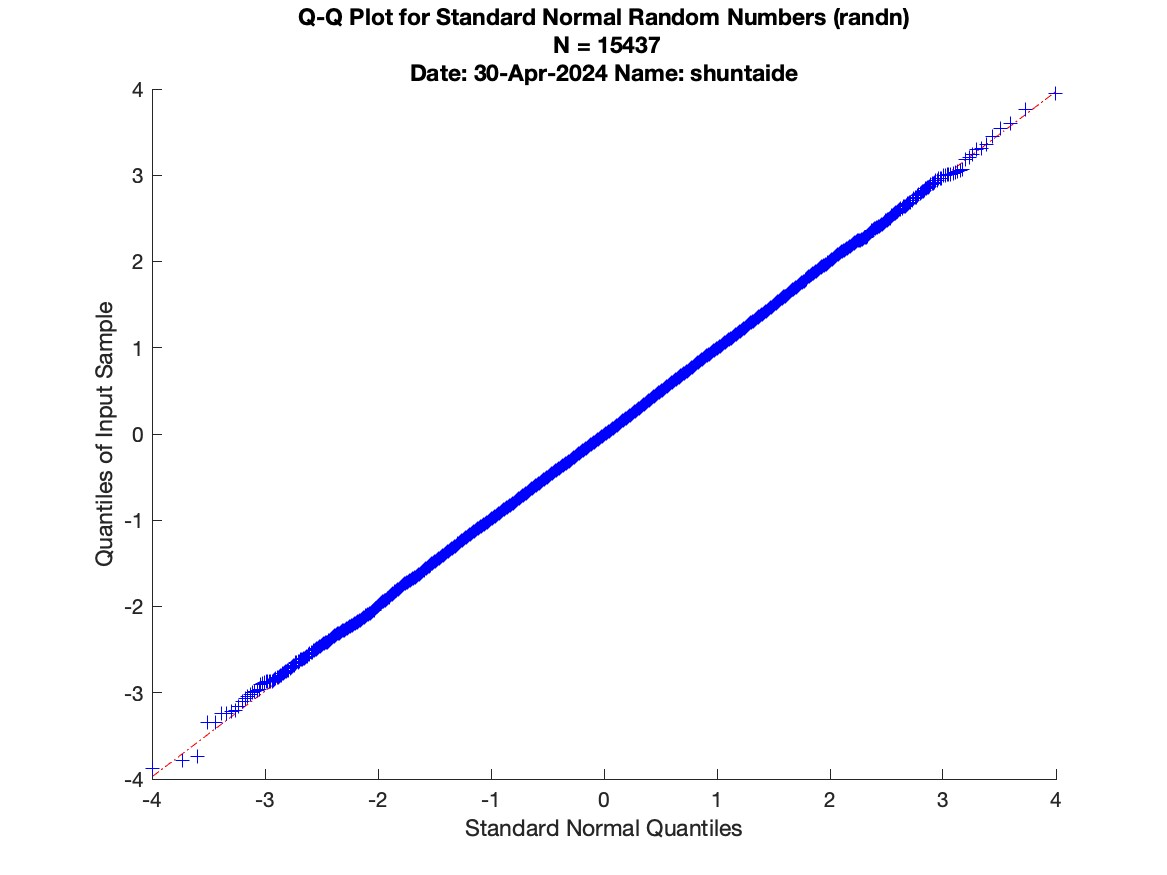
\includegraphics[width=0.8\linewidth]{src/figures/standard-normal/randn_qqpl_N=15437.jpg}
        \subcaption{QQプロット($N=15437$)}\label{fig:standard-normal-qqpl-15437}
    \end{subfigure}
    \begin{subfigure}{0.48\linewidth}
        \centering
        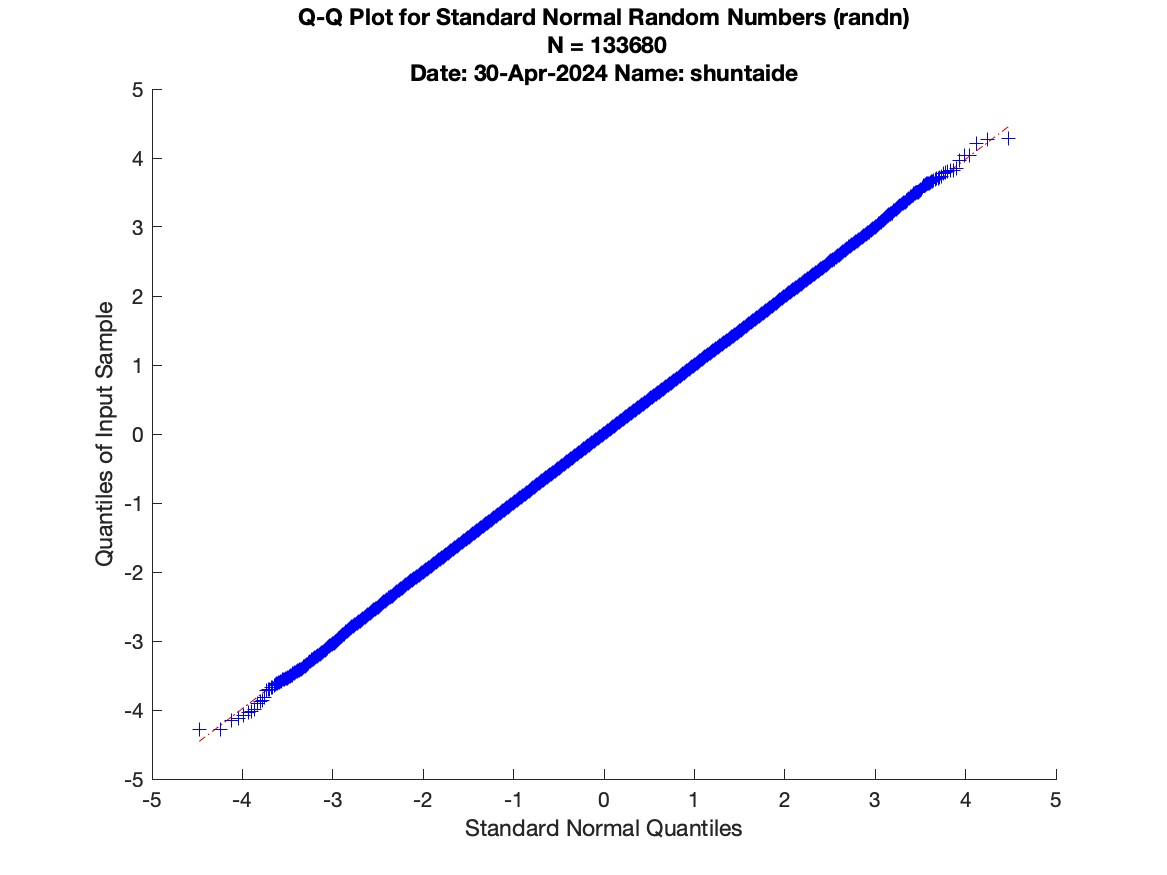
\includegraphics[width=0.8\linewidth]{src/figures/standard-normal/randn_qqpl_N=133680.jpg}
        \subcaption{QQプロット($N=133680$)}\label{fig:standard-normal-qqpl-133680}
    \end{subfigure}
    \caption{標準正規乱数の生成結果}\label{fig:standard-normal-random}
\end{figure}

図\ref{fig:standard-normal-qqpl-2511}、\ref{fig:standard-normal-qqpl-15437}、\ref{fig:standard-normal-qqpl-133680}は対応する$N$のQQプロットを示している。
$N$が大きくなるにつれ、直線へと近づき分布が標準正規分布に近づいていることがわかる。
$N$が小さいときは特に$-4$や$4$付近では直線が乱れているが、$N$が大きくなるにつれて直線に近づいている。

\subsubsection{BoxMuller法による標準正規乱数の生成結果}\label{subsubsec:box-muller-random}
BoxMuller法による標準正規乱数の生成結果を図\ref{fig:box-muller-random}に示す。
$N$は生成した乱数の数であり、横軸が生成された乱数の値、縦軸がその頻度を示している。
\ref{subsubsec:standard-normal-random}と同様に標準正規分布に近づいていることがわかる。

\begin{figure}
	\centering
	\begin{subfigure}{0.48\linewidth}
		\centering
		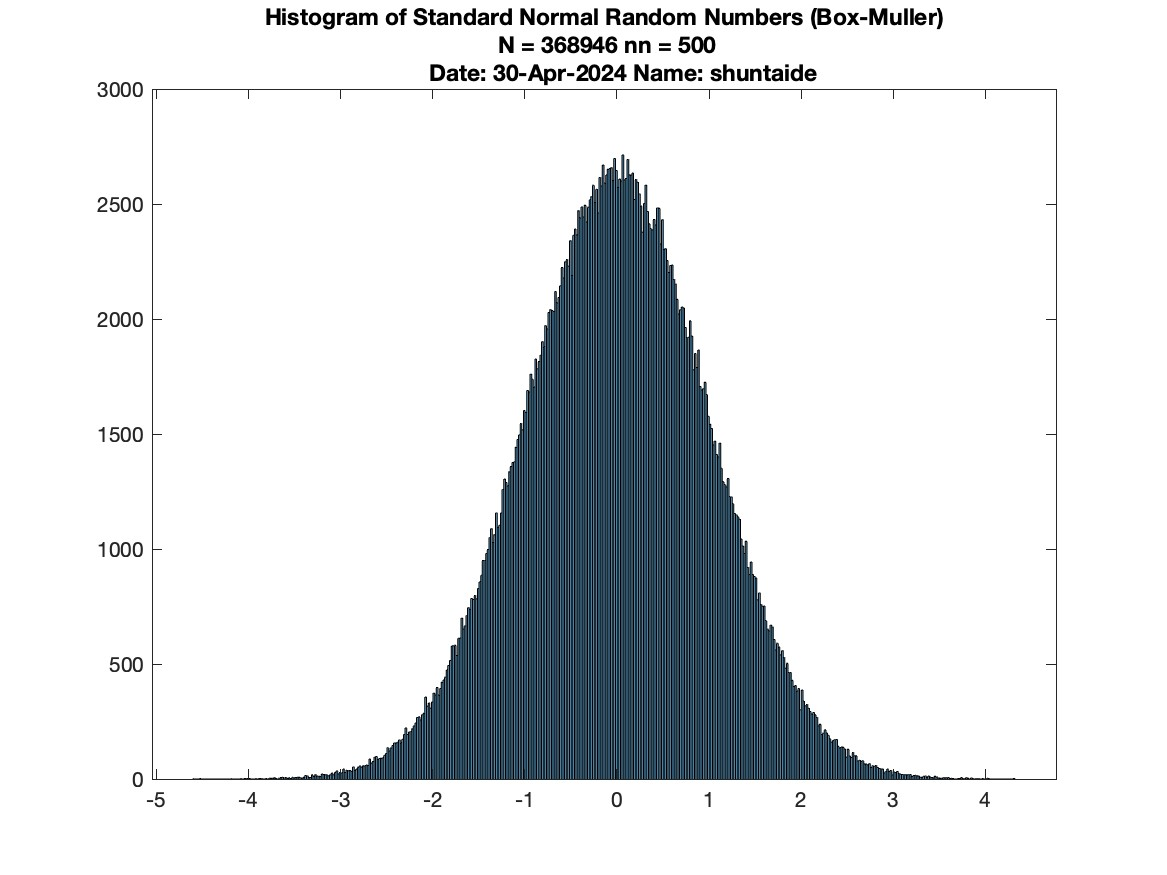
\includegraphics[width=0.8\textwidth]{src/figures/box-muller/Box-Muller_hist_N=368946_nn=500.jpg}
		\subcaption{ヒストグラム}
	\end{subfigure}
	\begin{subfigure}{0.48\linewidth}
		\centering
		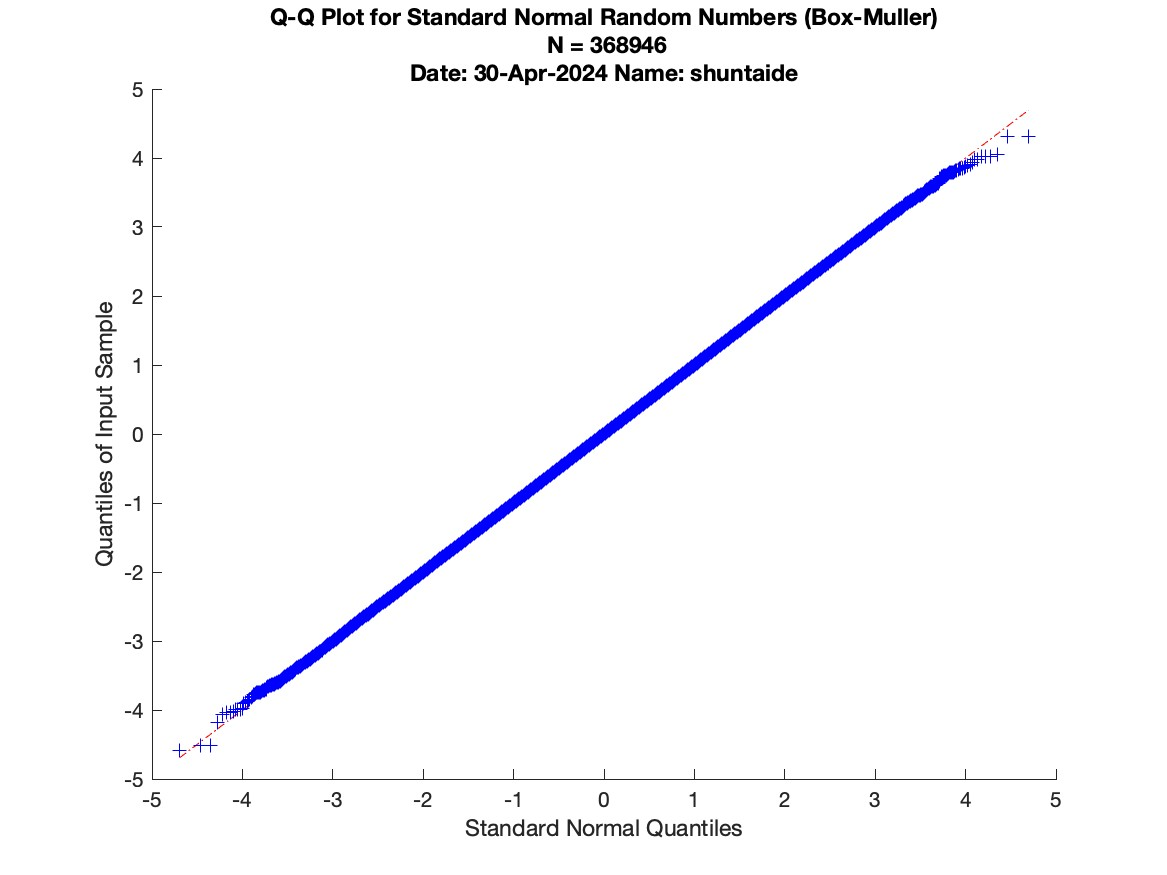
\includegraphics[width=0.8\textwidth]{src/figures/box-muller/Box-Muller_qqpl_N=368946.jpg}
		\subcaption{QQプロット}
	\end{subfigure}
	\caption{Box-Muller法による標準正規乱数の生成結果}\label{fig:box-muller-random}
\end{figure}


\subsubsection{逆関数法による標準正規乱数の生成結果}
逆関数法による標準正規乱数の生成結果を図\ref{fig:inverse-transform-random}に示す。
$N$は生成した乱数の数であり、横軸が生成された乱数の値、縦軸がその頻度を示している。
\ref{subsubsec:standard-normal-random}や\ref{subsubsec:box-muller-random}と同様に標準正規分布に近い分布が得られていることがわかる。

\begin{figure}
	\centering
	\begin{subfigure}{0.48\linewidth}
		\centering
		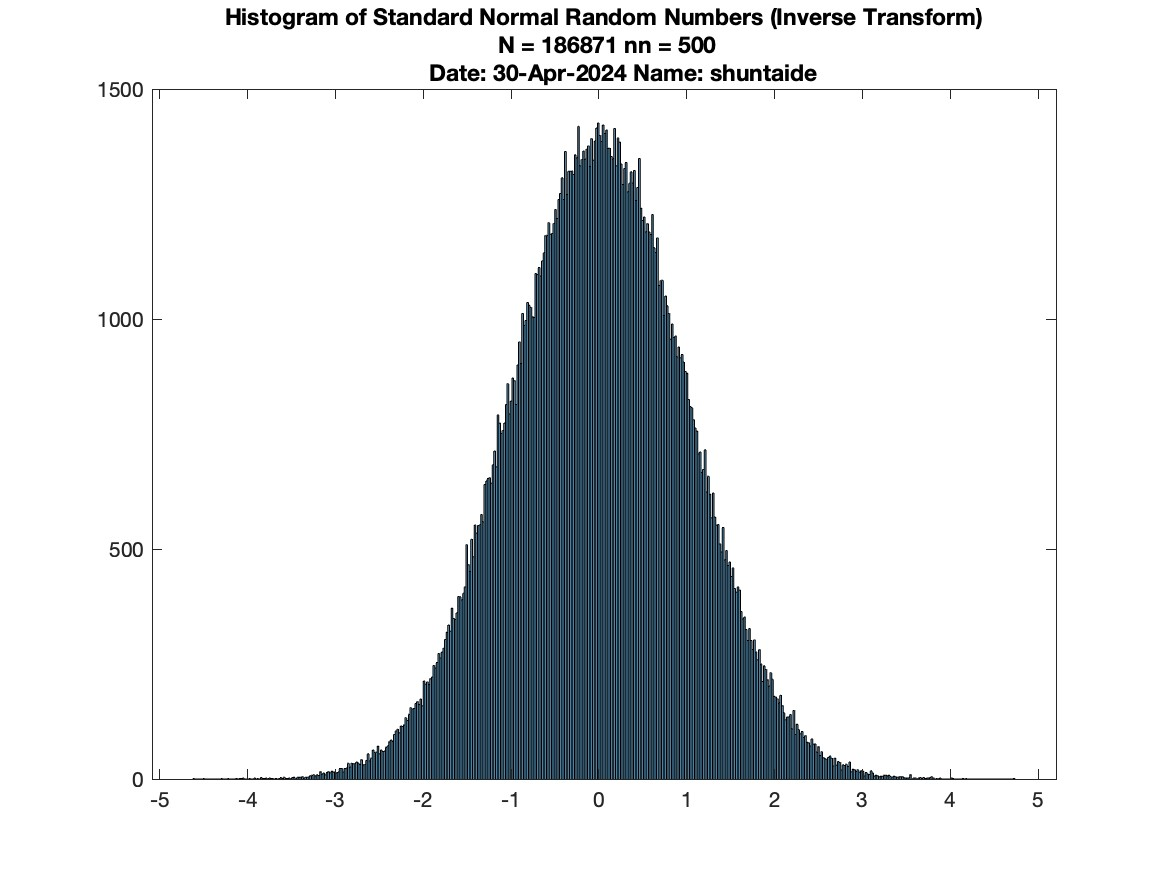
\includegraphics[width=0.8\linewidth]{src/figures/inverse-transform/Inverse_trans_hist_N=186871_nn=500.jpg}
		\subcaption{ヒストグラム}
	\end{subfigure}
	\begin{subfigure}{0.48\linewidth}
		\centering
		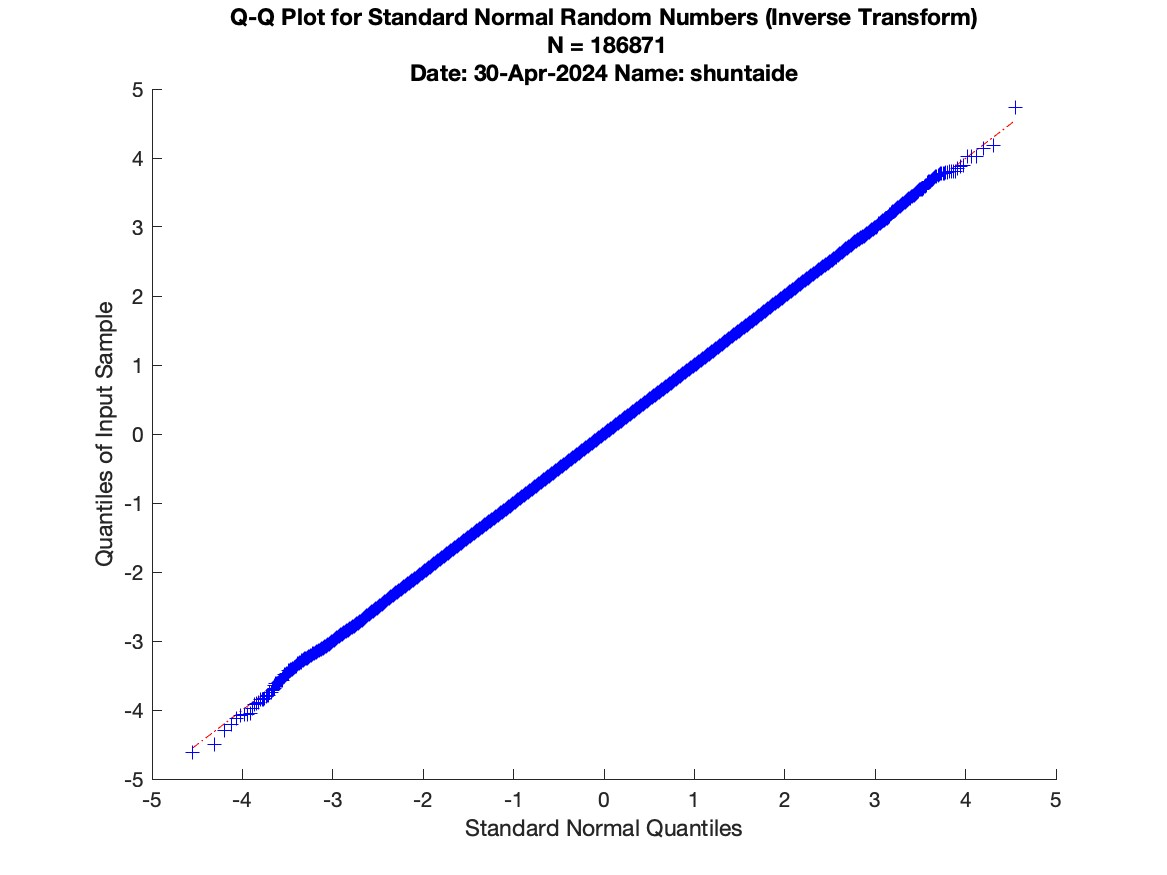
\includegraphics[width=0.8\linewidth]{src/figures/inverse-transform/Inverse_trans_qqpl_N=186871.jpg}
		\subcaption{QQプロット}
	\end{subfigure}
	\caption{逆変換法による標準正規乱数の生成結果}\label{fig:inverse-transform-random}
\end{figure}

